\documentclass[11pt]{beamer}
\usepackage[ngerman]{babel}
\usepackage{float}
\usepackage{graphicx}
\usepackage{caption}
\usepackage{hyperref}
\usepackage{cleveref}
\usepackage{fancyvrb}
\usepackage[%
  backend=bibtex,
  style=numeric-comp,
  citestyle=numeric-comp,
  isbn=false]{biblatex}
\AtEveryCitekey{\iffootnote{\clearfield{url}}{}}
\setbeamerfont{footnote}{size=\fontsize{4}{5}}
\captionsetup{justification=centering}
\addbibresource{bib.bib}
\author{Maximilian Heim\inst{1}}
\beamertemplatenavigationsymbolsempty
\beamerdefaultoverlayspecification{<+->}
\AtBeginSubsection[]
{
    \begin{frame}
        \frametitle{Table of Contents}
        \tableofcontents[currentsection,currentsubsection]
    \end{frame}
}
\usetheme{Madrid}
\usecolortheme{whale}
\institute[HS-AS]
{
  \inst{1}
  Hochschule Albstadt-Sigmaringen
}
\crefname{section}{Kapitel}{Kapitel}
\crefname{figure}{Abbildung}{Abbildung}
\title{Identitäts- und Berechtigungsmanagement}
\date[IT-GRC 2024]{IT-GRC Seminar, Juni 2024}
\begin{document}
\frame{\titlepage}
\begin{frame}
  \frametitle{Gliederung}
  \tableofcontents
\end{frame}
\section{Identitätsmanagement- und Berechtigungsmanagement}
\subsection{Identitätsmanagement}
\begin{frame}
  \frametitle{Identität im Kontext des Identitätsmanagements}
  \begin{itemize}
    \item Unterschiedliche Definitionen
    \item Identitätsmanagement: Digitale Identität
    \item Digitale Identität: Bezeichner, Zugangsdaten und Attribute
    \item Wichtig: Digitale Identitäten sind nicht nur Personen~\footfullcite{bertino2010identity}
  \end{itemize}
\end{frame}

\begin{frame}
  \frametitle{Digitale Identität}
  \begin{figure}[H]
    \centering
    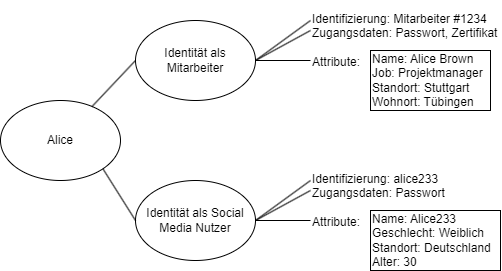
\includegraphics[width=0.7\textwidth]{assets/identity.png}
    \caption{Digitale Identität - Basierend auf Grafik 2.1 aus \glqq{}Identity Management Concepts, Technologies, and Systems\grqq{} von Elisa Bertino und Kenji Takahashi}
  \end{figure}
\end{frame}
\begin{frame}
  \frametitle{Identitätsmanagement}
  \begin{itemize}
    \item Management von digitalen Identitäten
    \item Gründe:
          \begin{itemize}
            \item Speicherung, Nutzung und Weitergabe von Identitätsinformationen
            \item Berechtigungsmanagement
          \end{itemize}
    \item Aufgabenbereiche:
          \begin{itemize}
            \item Prozesse (Identitätslebenszyklus)
            \item Technische Umsetzung (Speicherung, Weitergabe und Authentifizierung)
            \item Compliance mit Gesetzen und Standards
            \item Auditierung von Ist vs. Soll
          \end{itemize}
  \end{itemize}
\end{frame}

\begin{frame}
  \frametitle{Identitätslebenszyklus}
  \begin{figure}[H]
    \centering
    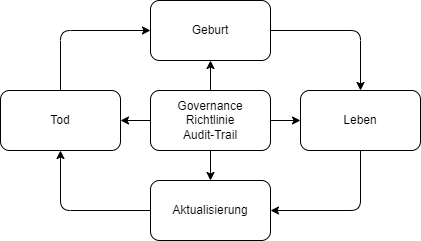
\includegraphics[width=0.6\textwidth]{assets/idlc.png}
    \caption{Identitätslebenszyklus - Basierend auf Grafik 2.3 aus \glqq{}Identity Management Concepts, Technologies, and Systems\grqq{} von Elisa Bertino und Kenji Takahashi}\label{fig:idlc}
  \end{figure}
\end{frame}

\begin{frame}<4->
  \frametitle{Identitätslebenszyklus}
  \begin{columns}
    \begin{column}{0.7\textwidth}
      \begin{figure}[H]
        \centering
        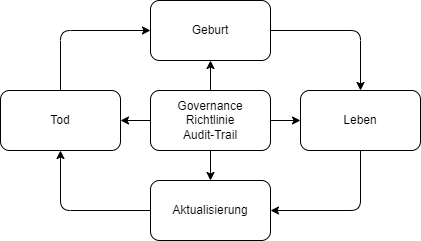
\includegraphics[width=0.6\textwidth]{assets/idlc.png}
        \caption{Identitätslebenszyklus - Basierend auf Grafik 2.3 aus \glqq{}Identity Management Concepts, Technologies, and Systems\grqq{} von Elisa Bertino und Kenji Takahashi}\label{fig:idlc}
      \end{figure}
    \end{column}
    \begin{column}{0.3\textwidth}
      \begin{itemize}
        \item Geburt: Datensammlung und Validierung, Zugangsdaten
        \item Leben: Authentifizierung, Weitergabe
        \item Aktualisierung: Änderungen, Zugangsdaten
        \item Tod: Kündigung, Löschung
        \item Governance: Richtlinien, Audit-Trail~\footfullcite{bertino2010identity}
      \end{itemize}

    \end{column}
  \end{columns}
\end{frame}

\subsection{Berechtigungsmanagement}
\begin{frame}
  \frametitle{Berechtigung}
  \begin{itemize}
    \item Kombination aus Ressource und Operation~\footfullcite{tsolkas2017}
    \item Beispiele:
          \begin{itemize}
            \item Wer darf Inhalte des \textbackslash{}\textbackslash{}ad.hochschule.de Verzeichnisses ändern?
            \item Wer darf in Azure DevOps Repositories löschen?
            \item Wer darf in AWS Zertifikate erstellen?
            \item Wer darf das Wohnheim in der Poststraße 22 betreten?
          \end{itemize}
  \end{itemize}
\end{frame}

\begin{frame}
  \frametitle{Berechtigungsmanagement}
  \begin{itemize}
    \item Management von Berechtigungen: Welche Nutzer oder IT-Systeme (digitale Identitäten) dürfen auf welche Ressourcen zugreifen?
    \item Gründe:
          \begin{itemize}
            \item PoLP/Principle of Least Privilege
            \item SoD/Funktionstrennung
            \item Rückverfolgbarkeit
          \end{itemize}
    \item Aufgaben:
          \begin{itemize}
            \item Berechtigungskonzept auf Unternehmen anpassen - RBAC, ABAC \ldots
            \item Technische Umsetzung (Authorisierung)
            \item Compliance mit Gesetzen und Standards
            \item Auditierung Ist vs. Soll
          \end{itemize}
  \end{itemize}
\end{frame}

\subsection{Identitäts- und Berechtigungsmanagement}

\begin{frame}
  \frametitle{Identitäts- und Berechtigungsmanagement-Systeme}
  \begin{figure}[H]
    \centering
    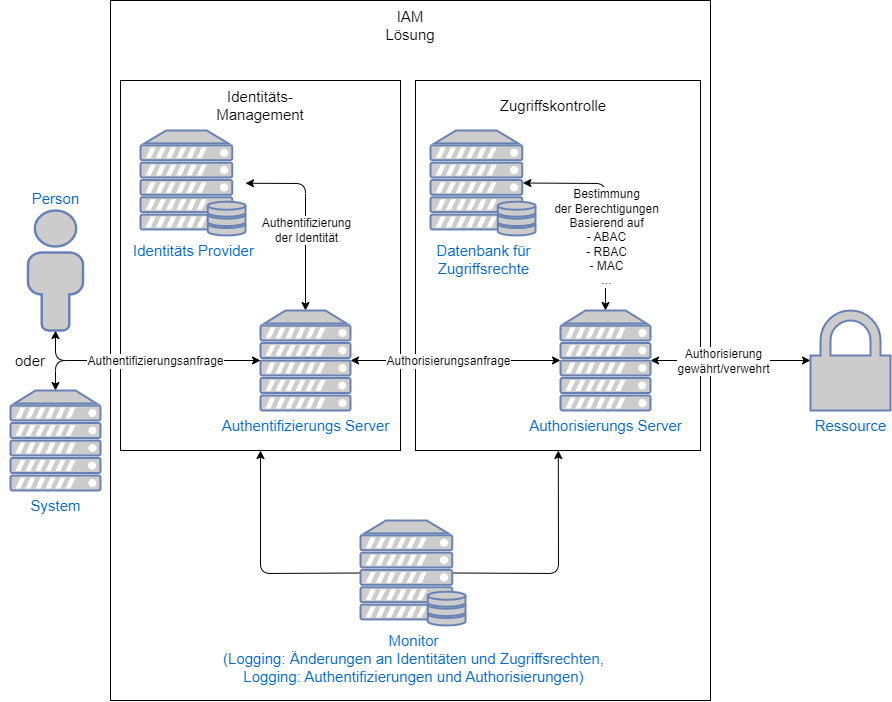
\includegraphics[width=0.7\textwidth]{assets/accessmanagement2.png}
    \caption{IAM System - Basierend auf Grafik 1 aus \glqq{}Identity and access management using distributed ledger technology: A survey\grqq{} von Fariba Ghaffari, Komal Gilani, Emmanuel Bertin und Noel Crespi}\label{figure:iam}
  \end{figure}
\end{frame}

\section{Betriebliches Identitäts- und Berechtigungsmanagement}

\subsection{Operative Aspekte}
\begin{frame}
  \frametitle{Operative Aspekte}
  \begin{itemize}
    \item CIO: Verantworlich für Prozesse und Technologien
    \item CISO: Bewertung der Prozesse, Überwachung der Compliance mit Datenschutzgesetzen und Sicherheitsstandards, Awareness Trainings, interne Audits...~\footfullcite{mont2010economics}
    \item IT-Betrieb: Implementierung und Wartung der involvierten Technik~\footfullcite{microsoft2024iamadmin}
    \item Personalabteilung: Identity-Lifecycle Management~\footfullcite{mohammed2017systematic}
    \item Helpdesk: Hilfe bei Authentifizierung und Authorisierung~\footfullcite{ylen2004centralized}
  \end{itemize}
\end{frame}

\subsection{Technische Aspekte}
\begin{frame}
  \frametitle{Technische Aspekte}
  \begin{itemize}
    \item Produkte von Konzernen wie Microsoft, SAP, IBM, Okta \ldots
          \begin{itemize}
            \item Neue Entwicklung: Cloud (IDaaS - Identity as a Service) im Gegensatz zu traditionellen On-Premise Lösungen~\footfullcite{kunz2014analyzing}
            \item Implementieren Technologien für optimale Umsetzung: Multi Faktor Authentifizierung (OTP, Biometrie), Single Sign On\ldots
            \item Unterstützen Prozesse: Lifecycle Management, Risikoanalyse, Audit-Management~\footfullcite{ibm2024verify}
            \item Integration von Service Providern: Active Directory, Microsoft Office, AWS, HR Anwendungen~\footfullcite{okta2024integrations}
          \end{itemize}
  \end{itemize}
\end{frame}

\begin{frame}
  \frametitle{Technische Aspekte}
  \begin{figure}[H]
    \centering
    \includegraphics<1>[width=0.9\textwidth]{assets/Entra.png}
    \caption{\only<1>{Microsoft Entra ID - von \url{https://www.microsoft.com/de-de/security/business/microsoft-entra}}}
  \end{figure}
\end{frame}

\subsection{Compliance Aspekte}

\begin{frame}
  \frametitle{Standards}
  \begin{itemize}
    \item ISO/IEC 24760: Identitätsmanagement (Konzepte und operative Strukturen)~\footfullcite{iso2019idm}
    \item ISO 27001: Annex A.9 definiert Zugangssteuerung~\footfullcite{kersten2020iso27001}
    \item IT-Grundschutz: BSI-Standard 200-1, ORP.4~\footfullcite{bsi20172001}\footfullcite{orp4}
  \end{itemize}
\end{frame}

\begin{frame}
  \frametitle{Rechtlich}
  \begin{itemize}
    \item EuroSOX (EU-Richtlinie 2006/43/EG): Berechtigungskontrolle, Funktionstrennung
    \item KonTraG (Gesetz zur Kontrolle und Transparenz im Unternehmensbereich): Risikomanagementsystem
    \item GoBD (Grundsätze zur ordnungsmäßigen Führung und Aufbewahrung von Büchern, Aufzeichnungen und Unterlagen in elektronischer Form sowie zum Datenzugriff): Berechtigungskontrolle, Nachvollziehbarkeit von Änderungen
    \item EU-DSGVO (EU- Datenschutzgrundverordnung) und BDSG (Bundesdatenschutzgesetz): Speicherung, Verarbeitung und Weitergabe von personenbezogenen Daten~\footfullcite{conta2017leitfaden}\footfullcite{eu2016}
  \end{itemize}
\end{frame}

\begin{frame}
  \frametitle{Fragen}
  \begin{itemize}
    \item Vielen Dank für eure Aufmerksamkeit!
    \item Fragen?
  \end{itemize}
\end{frame}

\begin{frame}[allowframebreaks]
  \frametitle{Literaturverzeichnis}
  \printbibliography
\end{frame}

\end{document}